%!TEX root = ../thesis.tex
\chapter{RGB-D图像的获取与融合}
\label{chap:rgbd}

\section{3D相机现状与分析}

\section{RGB-D相机}
\subsection{RGB-D相机原理与结构}
RGB-D相机获取深度的原理大致可以分为三种:
\begin{itemize}
\item Structure Light
\item Time of Flight(ToF)
\item Stereo
\end{itemize}

% @TODO: 加些原理图?
Structure Light获取深度信息的原理是通过激光发射器投射带有特定编码的结构光到物体表面后,由IR Camera采集,根据采集到的光信号量的变化来计算物体的深度。举一个形象的例子,将手电筒照向墙面,手电筒离墙面越远,墙面上所形成的光斑的直径就越大,所以可以通过光斑的直径来计算手电筒距离墙面的距离。ToF获取深度信息的原理是通过专有的传感器捕捉红外光发射到接收的飞行时间来计算物体的深度。Stereo是通过双摄像头拍摄物体,再通过特征点匹配,根据三角测量原理来计算物体的深度。

三种原理的深度相机各有其特点,采用Structure Light原理的深度相机一般精度比较高,但景深比较短并且受光线影响比较大,适合室内场景;ToF原理的深度相机获取深度图的精度和分辨率一般都比较低,但帧率高,并且具有一定的抗光照性能;Stereo获取深度精度适中,帧率相对来说较低,并且需要较强的计算性能,但抗光照能力强,适合室外场景。

本文所使用的RGB-D相机是Intel的Realsense SR300相机,SR300采用的结构光的原理获取深度,其内部结构如图\ref{fig:sr300}所示。
\begin{figure}[!ht]
  \centering
  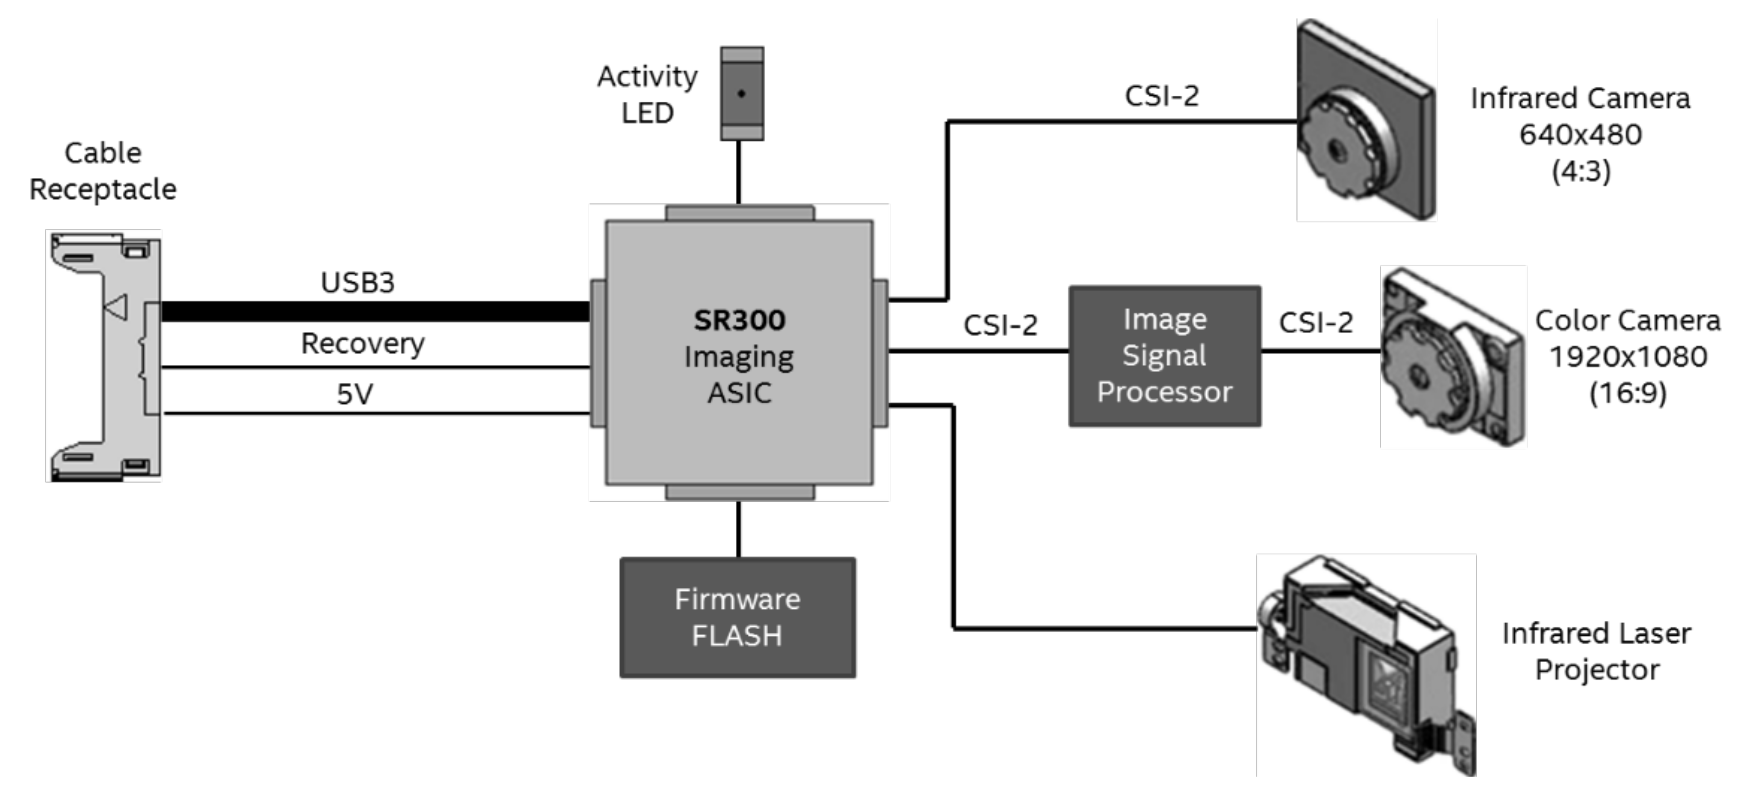
\includegraphics[width=12cm]{sr300}
  \caption{Realsense SR300内部结构图}
  \label{fig:sr300}
\end{figure}
从图\ref{fig:sr300}可以看出,SR300内部的传感器主要有彩色摄像头(Color Camera)、红外激光发射器(Infrared Laser Projector)和红外摄像头(Infrared Camera)。Color Camera是1920×1080像素的普通针孔摄像头,用来获取彩色图像;Infrared Laser Projector和Infrared Camera用来获取深度图像或者红外成像图,两种成像流程如图\ref{fig:capture_flow}所示。
\begin{figure}[!ht]
  \centering
  \subfloat[Depth Video Data Flow]{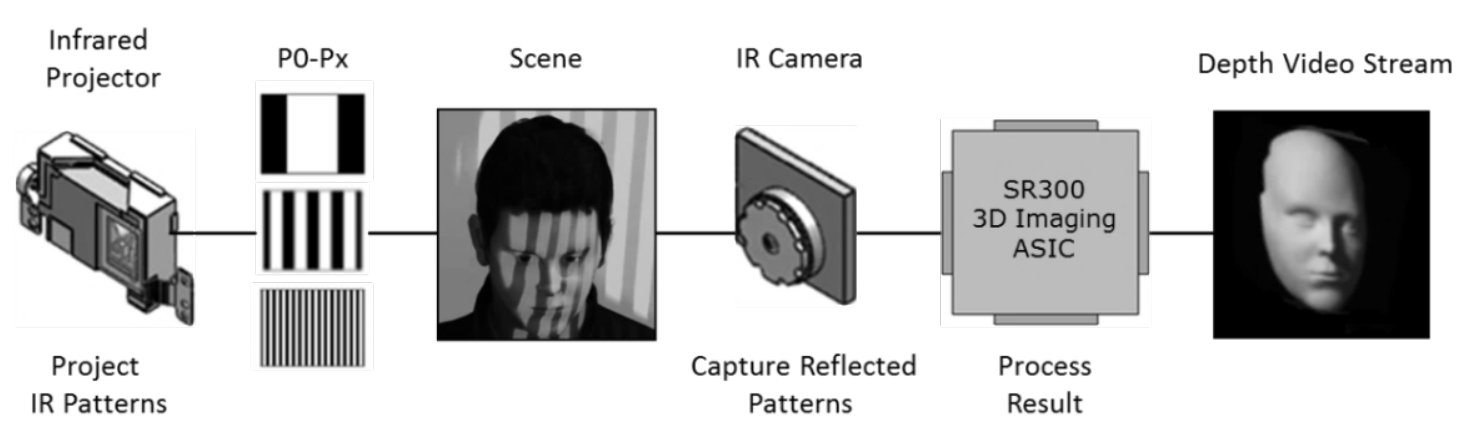
\includegraphics[width=12cm]{depth_flow}}
  \vfill
  \subfloat[IR Video Data Flow]{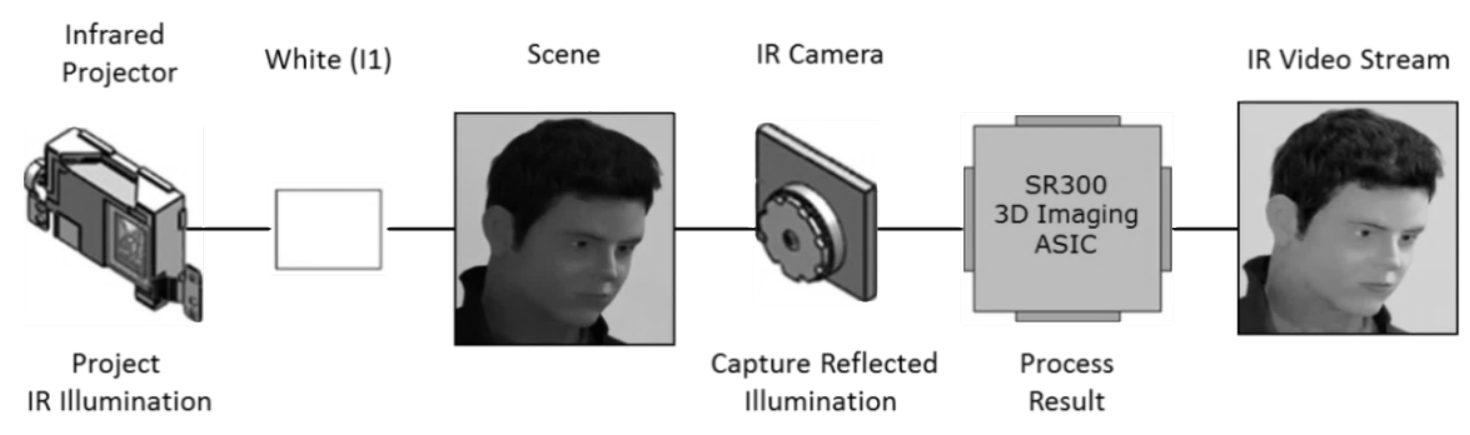
\includegraphics[width=12cm]{ir_flow}}
  \caption{Realsense SR300深度成像流程}
  \label{fig:capture_flow}
\end{figure}
其中当Infrared Laser Projector投射带有编码的结构光时,Infrared Camera可以获取深度图;当投射不带编码的红外光时,Infrared Camera可以获取红外成像图。正常使用时,往往设置Infrared Laser Projector投射带有编码的结构光来获取深度信息。因此,从RGB-D相机的使用来看,可以忽略其内部具体结构,将其看成由一个彩色摄像头和一个深度摄像头构成,其中彩色摄像获取彩色(RGB)信息,深度摄像头获取深度(depth)信息。

\subsection{RGB-D相机标定}
根据上文所述的RGB-D相机的结构,RGB-D相机的标定主要涉及到彩色摄像头内参和畸变的标定,深度摄像头内参和畸变的标定,以及彩色摄像头和深度摄像头之间位姿变换的标定。由于RGB-D相机是一种较为新颖的相机,所以市面上基本上没有较为成熟通用的标定RGB-D相机的方法以及对应的工具。因此本文针对所使用的Realsense SR300相机,设计了一套标定方法。
\subsubsection{RGB-D相机模型}
\begin{figure}[!ht]
  \centering
  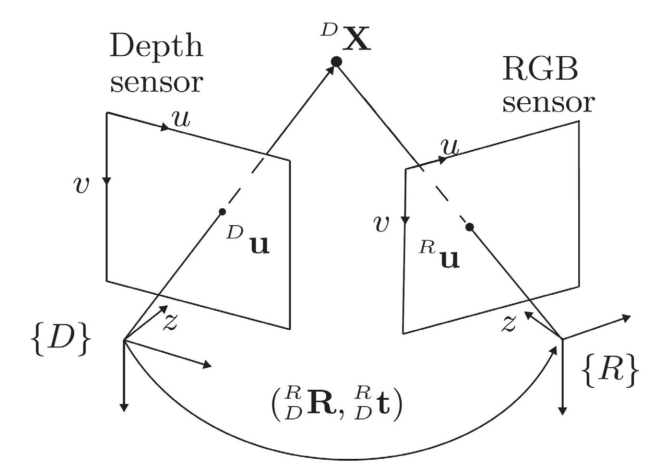
\includegraphics[width=8cm]{rgbd_model}
  \caption{RGB-D相机模型}
  \label{fig:rgbd_model}
\end{figure}
图\ref{fig:rgbd_model}展示了本文所使用的RGB-D相机的基本模型,其中彩色摄像头和深度摄像头都使用了针孔(pin-hole)相机模型\cite{Heikkila2000}。
%先考虑普通彩色相机的模型,彩色相机图像坐标系下一点$\tensor*[^R]{\bm{u}}{}:=[\prescript{R}{}{u},\prescript{R}{}{v}]^T$,其中上标$R$表示彩色相机(RGB),$\tensor*[^R]{\bm{u}}{}$对应的三维世界中的一点在彩色相机坐标系下表示为$\tensor*[^R]{\bm{X}}{}:=[\prescript{R}{}{x},\prescript{R}{}{y},\prescript{R}{}{z}]^T$。根据针孔相机模型有:
%\begin{equation}
%  \label{eq:r_cam_model}
%  \prescript{R}{}{z}{}\tensor[^R]{\bm{\tilde{u}}}{} = \tensor[^R]{\bm{K}}{}\tensor[^R]{\bm{X}}{}
%\end{equation}
%其中$\tensor[^R]{\bm{\tilde{u}}}{}$表示$\tensor[^R]{\bm{u}}{}$的齐次变换形式,彩色相机的内参矩阵$\tensor[^R]{\bm{K}}{}$的定义如下:
%\begin{equation}
%  \tensor[^R]{\bm{K}}{} := \left[
%    \begin{array}{ccc}
%      \prescript{R}{}{f}_u&0&\prescript{R}{}{u}_0 \\
%      0&\prescript{R}{}{f}_v&\prescript{R}{}{v}_0 \\
%      0&0&1
%    \end{array}
%  \right]
%\end{equation}
%其中$\prescript{R}{}{f}_u$和$\prescript{R}{}{f}_v$分别表示彩色相机在图像坐标轴上的焦距(以像素为单位),$\prescript{R}{}{u}_0$,$\prescript{R}{}{v}_0$表示彩色相机光心在图像平面的投影中心。
先考虑普通针孔相机的模型,相机图像坐标系下一点$\bm{u}:=[u,v]^T$,对应的三维世界中的一点在相机坐标系下表示为$\bm{X}:=[x,y,z]^T$。根据针孔相机模型有:
\begin{equation}
  \label{eq:cam_model}
  z\bm{\tilde{u}} = \bm{K}\bm{X}
\end{equation}
其中$\bm{\tilde{u}}$表示$\bm{u}$的齐次变换形式,彩色相机的内参矩阵$\bm{K}$的定义如下:
\begin{equation}
  \bm{K} := \left[
    \begin{array}{ccc}
      f_u&0&u_0 \\
      0&f_v&v_0 \\
      0&0&1
    \end{array}
  \right]
\end{equation}
其中$f_u$和$f_v$分别表示彩色相机在图像坐标轴上的焦距(以像素为单位),$u_0$和$v_0$表示彩色相机光心在图像平面的投影中心。

公式\ref{eq:cam_model}还未考虑镜头的畸变,为了提高相机的精度,现引入径向畸变(radial distortion)和切向畸变(tangential distortion):
\begin{itemize}
\item 径向畸变是由相机透镜的不完善和表面曲率存在误差造成的,径向畸变的数学模型可以表示为:
  \begin{equation}
    \label{eq:radial}
    \left\{
      \begin{array}{ccc}
        \hat{x}&=&\bar{x}(1 + k_1r^2 + k_2r^4 + k_3r^6)\\
        \hat{y}&=&\bar{y}(1 + k_1r^2 + k_2r^4 + k_3r^6)\\
      \end{array}
    \right.
  \end{equation}
  其中
  \begin{align}
    \bar{x} =& x/z\\
    \bar{y} =& y/z\\
    r  =& \sqrt{\bar{x}^2 + \bar{y}^2}
  \end{align}
  $\bar{x}$,$\bar{y}$表示点$\bm{X}$在归一化平面上的坐标,$\hat{x}$,$\hat{y}$表示修正径向畸变后的的坐标,$k_1$,$k_2$,$k_3$表示径向畸变的参数。
\item 切向畸变是由于相机透镜与图像平面不平行造成的,其数字模型可以表示为:
  \begin{equation}
    \label{eq:trang}
    \left\{
      \begin{array}{ccc}
        \hat{x}&=&\bar{x} + (2p_1\bar{x}\bar{y} + p_2(r^2 + 2\bar{x}^2))\\
        \hat{y}&=&\bar{y} + (p_1(r^2 + 2\bar{y}^2) + 2p_2\bar{x}\bar{y})\\
      \end{array}
    \right.
  \end{equation}
  其中$p_1$,$p_2$是切向畸变的参数。
\item 结合公式\ref{eq:radial}和\ref{eq:trang}可以得到修正径向畸变和切向畸变的模型:
  \begin{equation}
    \label{eq:dist}
    \left\{
      \begin{array}{ccc}
        \hat{x}&=&\bar{x}(1 + k_1r^2 + k_2r^4 + k_3r^6) + (2p_1\bar{x}\bar{y} + p_2(r^2 + 2\bar{x}^2))\\
        \hat{y}&=&\bar{y}(1 + k_1r^2 + k_2r^4 + k_3r^6) + (p_1(r^2 + 2\bar{y}^2) + 2p_2\bar{x}\bar{y})\\
      \end{array}
    \right.
  \end{equation}
\end{itemize}
通过以上分析,根据公式\ref{eq:cam_model}和\ref{eq:dist}可以推导出带有畸变的针孔相机模型:
\begin{equation}
  \label{eq:dist_cam_model}
  \left\{
    \begin{array}{ccc}
      u&=&f_u(\bar{x}(1 + k_1r^2 + k_2r^4 + k_3r^6) + (2p_1\bar{x}\bar{y} + p_2(r^2 + 2\bar{x}^2))) + u_0\\
      v&=&f_v(\bar{y}(1 + k_1r^2 + k_2r^4 + k_3r^6) + (p_1(r^2 + 2\bar{y}^2) + 2p_2\bar{x}\bar{y})) + v_0
    \end{array}
  \right.
\end{equation}
为方便起见,记$\bm{d}:=[k_1,k_2,p_1,p_2,k_3]^T$,定义函数
\begin{equation}
  f_{undist}(\bm{d}, \bm{X}):=\left[
    \begin{array}{ccc}
      \bar{x}(1 + k_1r^2 + k_2r^4 + k_3r^6) + (2p_1\bar{x}\bar{y} + p_2(r^2 + 2\bar{x}^2))\\
      \bar{y}(1 + k_1r^2 + k_2r^4 + k_3r^6) + (p_1(r^2 + 2\bar{y}^2) + 2p_2\bar{x}\bar{y})\\
      1
    \end{array}
  \right]
\end{equation}
则公式\ref{eq:dis_cam_model}可简化为:
\begin{equation}
  \tilde{\bm{u}} = \bm{K}\cdot f_{undist}(\bm{d}, \bm{X})
\end{equation}
其中需要标定的参数有相机内参矩阵$\bm{K}$(包含未知参数$f_u$,$f_v$,$u_0$,$v_0$)以及畸变参数$\bm{d}$(包含未知参数$k_1$,$k_2$,$p_1$,$p_2$,$k_3$),共9个参数。

明确了针孔相机的数学模型后,很容易推出SR300的相机模型:
\begin{equation}
  \label{eq:rgbd_cam_model}
  \left\{
    \begin{array}{ccc}
      \tensor*[^R]{\tilde{\bm{u}}}{}&=&\tensor*[^R]{\bm{K}}{}\cdot f_{undist}(\tensor*[^R]{\bm{d}}{},\tensor*[^R]{\bm{X}}{})\\
      \tensor*[^D]{\tilde{\bm{u}}}{}&=&\tensor*[^D]{\bm{K}}{}\cdot f_{undist}(\tensor*[^D]{\bm{d}}{},\tensor*[^D]{\bm{X}}{})\\
      \tensor*[^R]{\bm{X}}{} &=& \tensor*[^R_D]{\bm{R}}{}\tensor*[^D]{\bm{X}}{} + \tensor*[^R_D]{\bm{t}}{}
    \end{array}
  \right.
\end{equation}
其中左上标$\{R\}$表示SR300相机中的彩色相机(RGB),$\{D\}$表示SR300相机中的深度相机(Depth),$\tensor*[^R_D]{\bm{R}}{}$和$\tensor*[^R_D]{\bm{t}}{}$表示了彩色相机坐标系和深度相机坐标系之间的齐次变换关系。

\section{对偶RGB-D相机}

\subsection{对偶RGB-D相机原理与结构}

\subsection{深度图像融合算法}

\subsection{对偶RGB-D相机标定}